\documentclass[border=2pt]{standalone}

\usepackage{tikz}
    \usetikzlibrary{math, calc}
\usepackage{siunitx}

\begin{document}
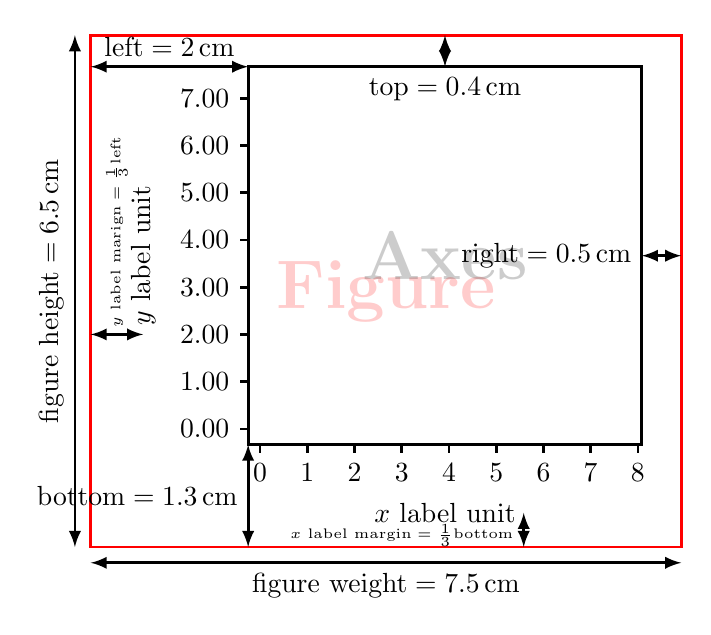
\begin{tikzpicture}[line width=1pt, scale=1]
    \tikzmath{
        \figweight=7.5;
        \figheight=6.5;
        \axleft=2;
        \axright=0.5;
        \axbottom=1.3;
        \axtop=0.4;
        \axweight=\figweight-\axleft-\axright;
        \axheight=\figheight-\axbottom-\axtop;
        \xlabelmargin=\axbottom/3;
        \ylabelmargin=\axleft/3;
    }

    \coordinate (O) at (0, 0);
    \draw [red] (O) rectangle ++(\figweight, \figheight);
    \node [red, opacity=0.2] at (\figweight/2, \figheight/2) {\bfseries\fontsize{65pt}{0}\selectfont Figure};
    \draw ($ (O) + (\axleft, \axbottom) $) rectangle ($ (O) + ({\figweight-\axright}, {\figheight-\axtop}) $);
    \node [opacity=0.2] at (\axleft+\axweight/2, \axbottom+\axheight/2) {\bfseries\fontsize{55pt}{0}\selectfont Axes};

    % x label
    \node at (\axleft+\axweight/2, \xlabelmargin) {$ x~\mathrm{label}~\unit{unit}$};
    \draw [latex-latex] ([xshift=1cm] \axleft+\axweight/2, 0) -- ++(0, \xlabelmargin) node [midway, left, yshift=-2pt] {\tiny  $ x~\mathrm{label~margin} = \frac{1}{3}\mathrm{bottom} $};

    % y label
    \node [rotate around={90:(0, 0)}] at (\ylabelmargin, \axbottom+\axheight/2) {$ y~\mathrm{label}~\unit{unit} $};
    \draw [latex-latex] ([yshift=-1cm] 0, \axbottom+\axheight/2) -- ++(\ylabelmargin, 0) node [midway, rotate=90, xshift=1.3cm] {\tiny $ y~\mathrm{label~marign} = \frac{1}{3}\mathrm{left} $};

    % figure size indicator
    \draw [latex-latex] ($ (O) + (-0.2, 0) $) -- ++(0, \figheight);
    \node [rotate around={90:(0, 0)}] at (-0.5, \figheight/2) {$ \mathrm{figure~height} = \qty{\figheight}{\centi\meter} $};
    \draw [latex-latex] ($ (O) + (0, -0.2) $) -- ++(\figweight, 0)
    node [below, midway] {$ \mathrm{figure~weight} = \qty{\figweight}{\centi\meter} $};

    % axes size indicator
    % 左侧
    \draw [latex-latex] (0, \figheight-\axtop) -- (\axleft, \figheight-\axtop)
    node [above, midway] {$ \mathrm{left} = \qty{\axleft}{\centi\meter} $};
    \foreach \i in {0, ..., 7}{%
            \draw ([yshift=0.2cm] \axleft, \axbottom+\i*0.6) -- ++(-3pt, 0) node [left] {\ensuremath{\i.00}};
        }
    % 底部
    \draw [latex-latex] (\axleft, 0) -- (\axleft, \axbottom)
    node [left, midway] {$ \mathrm{bottom} = \qty{\axbottom}{\centi\meter} $};
    \foreach \i in {0, ..., 8}{%
            \draw ([xshift=0.15cm] \axleft+\i*0.6, \axbottom) -- ++(0, -3pt) node [below] {\ensuremath{\i}};
        }
    % 顶部
    \draw [latex-latex] (\axleft+\axweight/2, \figheight) -- (\axleft+\axweight/2, \figheight-\axtop)
    node [below] {$ \mathrm{top} = \qty{\axtop}{\centi\meter} $};
    % 右侧
    \draw [latex-latex] (\figweight, \axbottom+\axheight/2) -- (\figweight-\axright, \axbottom+\axheight/2)
    node [left] {$ \mathrm{right} = \qty{\axright}{\centi\meter} $};
\end{tikzpicture}
\end{document}